\documentclass{article}
\textheight 23.5cm \textwidth 15.8cm
%\leftskip -1cm
\topmargin -1.5cm \oddsidemargin 0.3cm \evensidemargin -0.3cm
%\documentclass[final]{siamltex}

\usepackage{verbatim}
\usepackage{fancyhdr}
\usepackage{amssymb,ctex}
\usepackage{mathrsfs}
\usepackage{latexsym,amsmath,amssymb,amsfonts,epsfig,graphicx,cite,psfrag}
\usepackage{eepic,color,colordvi,amscd}
\usepackage{enumerate}
\usepackage{enumitem}
\usepackage{booktabs}
\usepackage{graphicx}
\usepackage{float}
\usepackage{wrapfig}
\usepackage{multirow}
\usepackage{subfigure}
\usepackage{diagbox}


\title{USTC\_CG HW3 PoissonImageEditing}
\author{张继耀,PB20000204}

\begin{document}
	\maketitle
	
	\tableofcontents
	
	\section {问题介绍}
	\subsection{主要目的}
	
	\begin{itemize}
		\item 实现 Poisson Image Editing 算法
	\end{itemize}
	
	\begin{itemize}
		\item 实现多边形光栅化的扫描线转换算法
	\end{itemize}
	
	\begin{itemize}
		\item 学习使用Eigen库、OpenCV
	\end{itemize}
	\begin{itemize}
	\item 通过矩阵预分解实现实时拖动区域显示结果
    \end{itemize}
	
		
	\section{算法设计}
	
	\subsection{程序框架}
	
	下面我们首先给出整个项目的类视图
	
		\begin{figure}[H]
		\begin{center}
			
			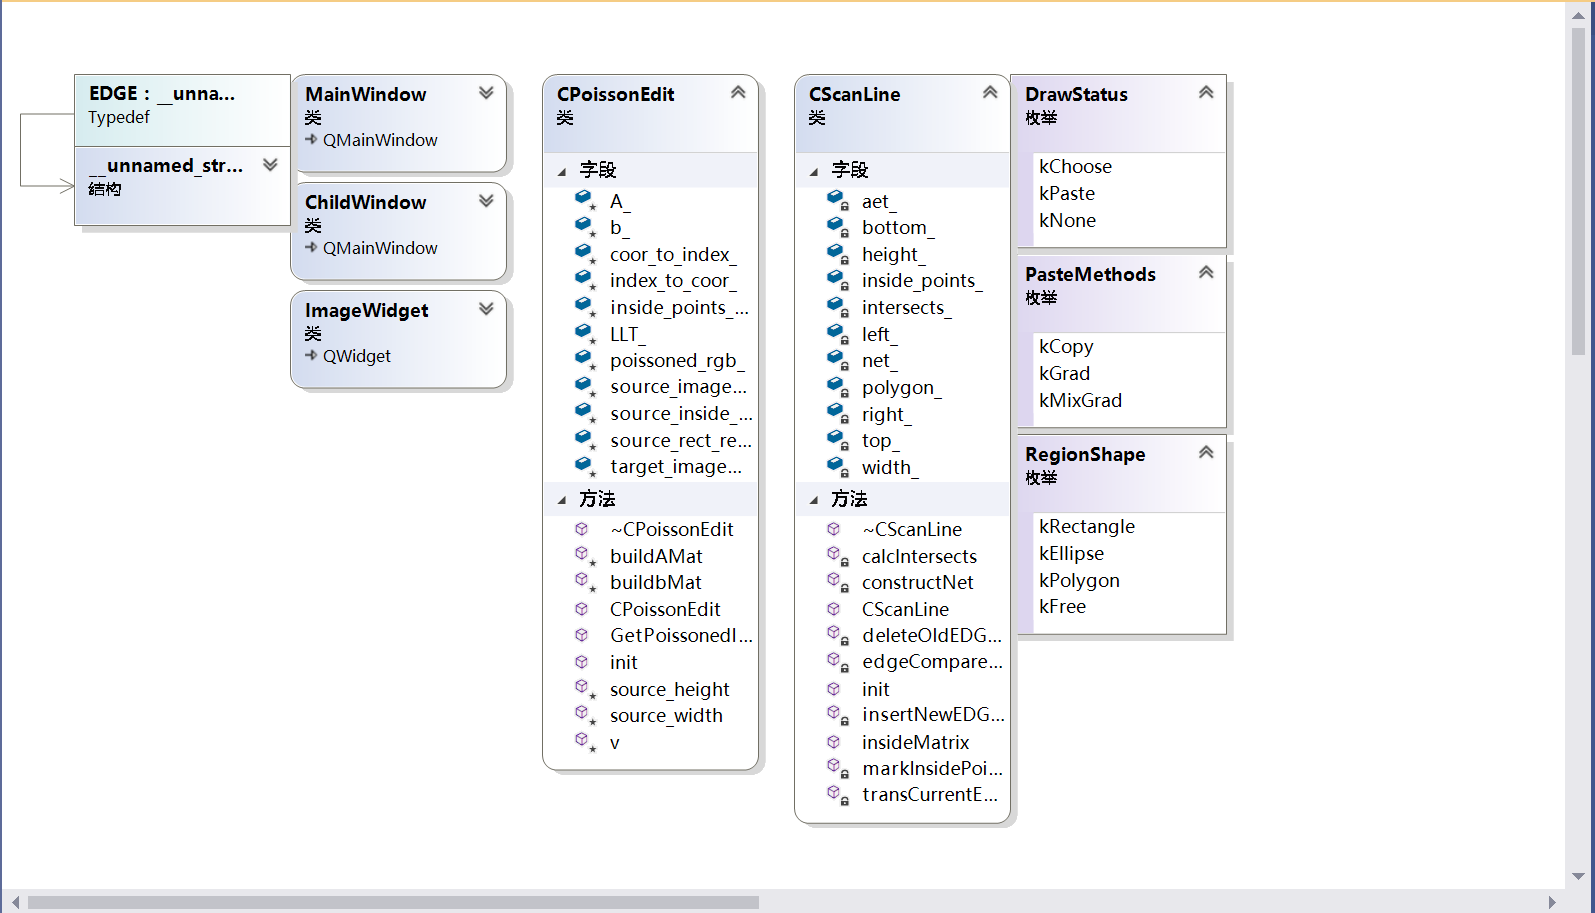
\includegraphics[width=18cm,height=10cm]{shitu}
			
			\caption{项目的类视图} \label{shitu.label}
		\end{center}
	\end{figure}
	

	
	\subsection{Poisson Image Editing 算法}
	
	该算法最初由Patrick Pérez、Michel Gangnet和Andrew Blake于2003年提出,可以在保持图像连续性的同时,将一张图像的内容嵌入到另一张图像中。
	
	该算法将原图像目标区域的梯度与被粘贴图像中的实际梯度相匹配,求解以下方程来实现图像融合:
		$$	\left\{ 
	\begin{array}{lc}
		min_f\iint_{\Omega}\left\vert \nabla f  \right\vert^2, f|_{\partial \Omega}=f^{\ast}|_{\partial \Omega}\\
		\Delta f=0 \enspace over \enspace \Omega , f|_{\partial \Omega}=f^{\ast}|_{\partial \Omega}\\
	\end{array}
	\right.$$
	
	在本问题中,求解图像的像素点事实上是一个离散的问题,转化成以下方程:
	
	 $$ \forall p\in \Omega, \left\vert N_p \right\vert f_p - \sum\limits_{q\in N_p \cap \Omega}f_q = \sum\limits_{q\in N_p \cap \partial \Omega}f^{\ast}_q + \sum\limits_{q\in N_p}v_{pq}$$
	 
	 其中 $v=\nabla g$为向量场,$g$为图像的像素点。$N_p$表示与像素点$p$相邻的四个像素集合。注意以上方程在内部时可以有更简单的形式。
	 
	  $$  \left\vert N_p \right\vert f_p - \sum\limits_{q\in N_p }f_q =  \sum\limits_{q\in N_p}v_{pq}$$
	  
	  论文\cite{PIE}中给出了两种选择梯度场的方法,一种是完全使用原图像的内部梯度
	  $$\forall \left< p, q \right>,v_{pq}=g_p-g_q$$
	  另一种是用混合梯度:
	 	$$   \forall x\in \Omega,v(x)=\left\{ 
	 \begin{array}{lc}
	 	\nabla f^{\ast}(x),\left\vert \nabla f^{\ast}(x) \right\vert > \left\vert \nabla g^{\ast}(x) \right\vert    \\
	 	\nabla g^{\ast}(x), \enspace otherwise    \\
	 \end{array}
	 \right.$$
	 
	 对图像的每个像素点列出以上的方程,就得到了一个线性方程组。系数矩阵A是一个稀疏矩阵,每行至多有5个非零元素。于是这个问题实质上又变成了解线性方程组的问题。
	
	
	\subsection{矩阵预分解}
	
	如果我们希望让用户在拖动时实时得到处理后的结果,就要采用矩阵预分解的方法。因为对于线性方程组$AX=b$,每次的矩阵$A$都是相同的(原图信息)。每次改变的事实上只是边界的信息,对矩阵$A$采取预分解可大大提高效率。
	
	在用户点击菜单时后台进行预分解,即可节省时间来实现实时拖动。这样能让用户体验更好。
	
	对于本问题,构造的矩阵A事实上是对称正定的。对称较易看出,因为两个点若为邻居一定是互为邻居的。正定则是因为矩阵的对角元元素都是大于0的。
	
	因此我们可以采用LLT方法进行预分解,这个方法的效率是最高的。
	
	\subsection{多边形扫描线算法}
	以下是扫描线算法的具体步骤:
	
	\begin{itemize}
	\item 首先得到多边形对应的y坐标的最小值与最大值
	\end{itemize}

	\begin{itemize}
	\item 然后从多边形的最低顶点开始,依次向上递增扫描线的位置
	 \subitem 若共享顶点的两条边分别落在扫描线两边,交点只算一个
	\subitem 若共享顶点的两条边落在扫描线同一边,交点算两个或零个
    \end{itemize}

	\begin{itemize}
	\item 求出扫描线与多边形的交点并排序
    \end{itemize}


	\begin{itemize}
	\item 将得到的顶点配对,每对顶点之间的点为内点
    \end{itemize}

	\begin{itemize}
	\item 重复以上步骤,得到多边形内部所有点
    \end{itemize}
	
	
	
	\section{结果展示}
	
	 \subsection{程序界面}
	
	\begin{figure}[H]
		\begin{center}
			
			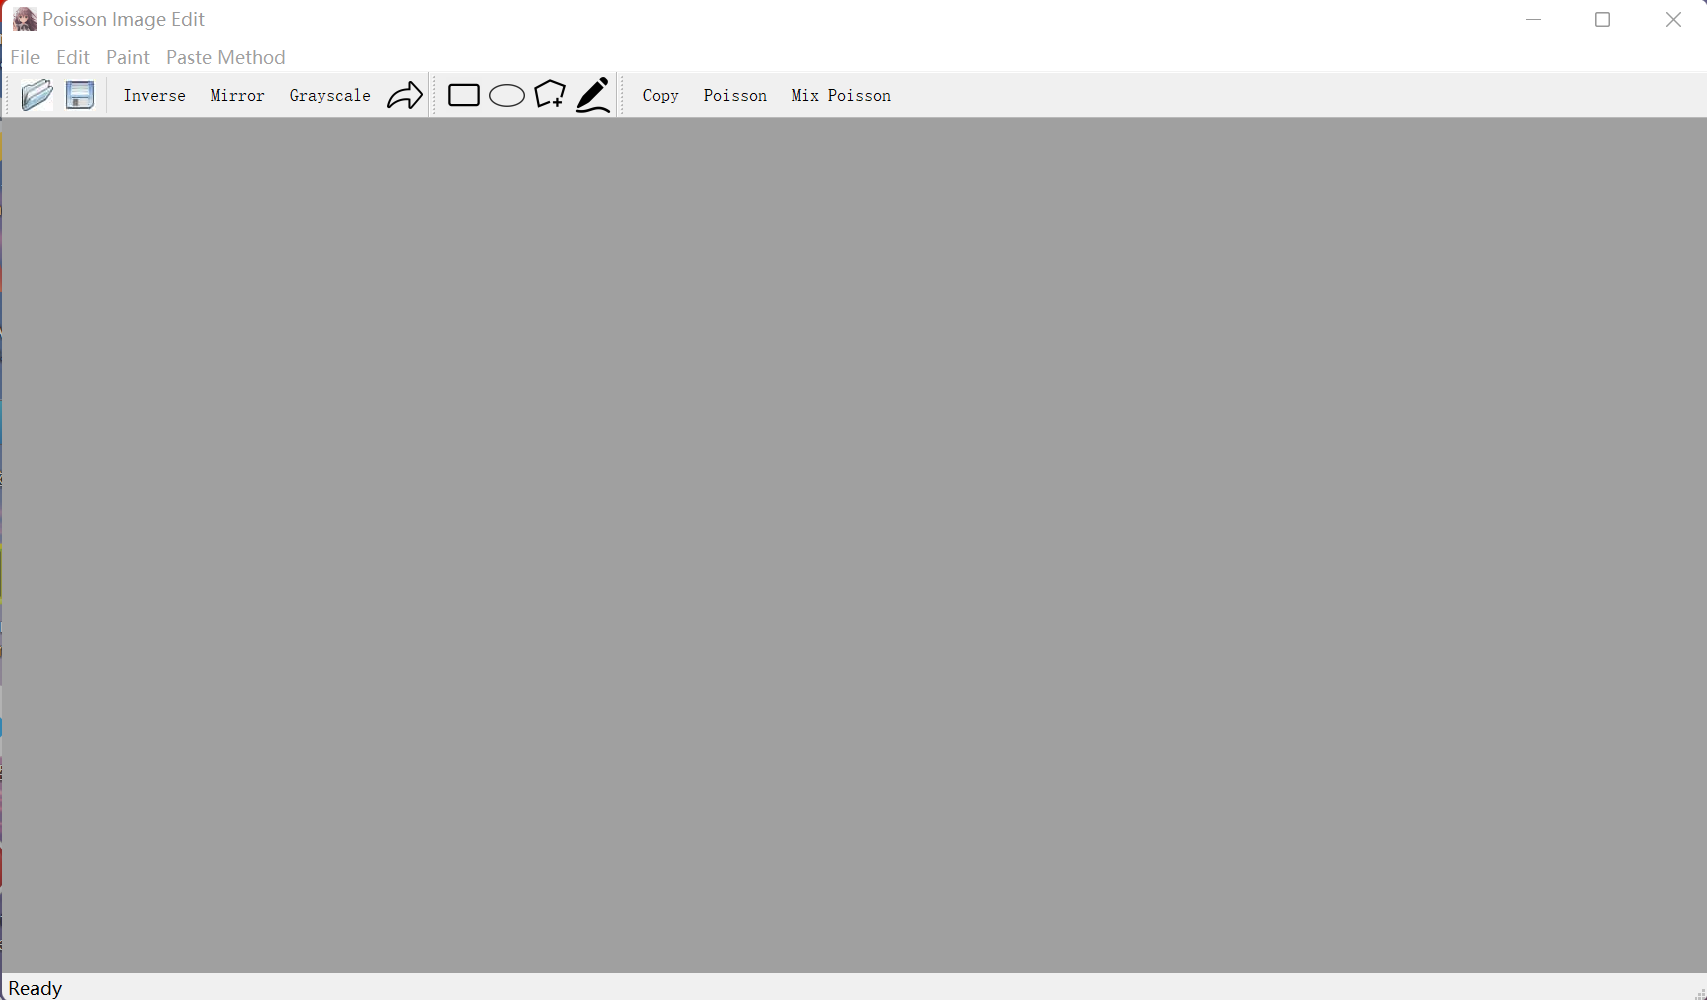
\includegraphics[width=13cm,height=8cm]{jiemian}
			
			\caption{程序界面} \label{jiemian.label}
		\end{center}
	\end{figure}
	
     \subsection{功能讲解}
     
      	\begin{itemize}
     	\item 最左边的图标是打开、保存图片, Redo可以恢复图片原始的样子,Inverse、Mirror、Grayscale可以对图像直接处理
     \end{itemize}

     \begin{itemize}
     	\item 中间的矩形、椭圆、多边形是选择划线区域的方式,用户可自由选择所划的区域。选择多边形方式时,双击鼠标左键代表结束选取。
     \end{itemize}
     \begin{itemize}
     	\item 最右边是选择复制的方式,依次为:直接像素粘贴、内部梯度粘贴、混合梯度粘贴
     \end{itemize}
     \begin{itemize}
     	\item 交互时,先选中要复制的图像,划出要复制的区域,再选中目标图像,选择复制方式,然后直接拖动鼠标即可实时得到结果。
     \end{itemize}
 
   \subsection{实验结果}
   
    \subsubsection{选择不同区域}
    
    选择矩形区域时
    
    	\begin{figure}[H]
    	\begin{center}
    		
    		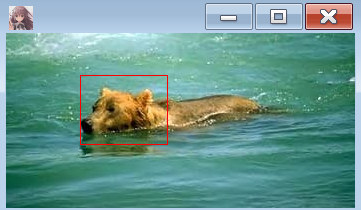
\includegraphics[width=6cm,height=4cm]{rect1}
    		
    		\caption{所选区域} \label{rect1.label}
    	\end{center}
    \end{figure}

	\begin{figure}[H]
	\begin{center}
		
		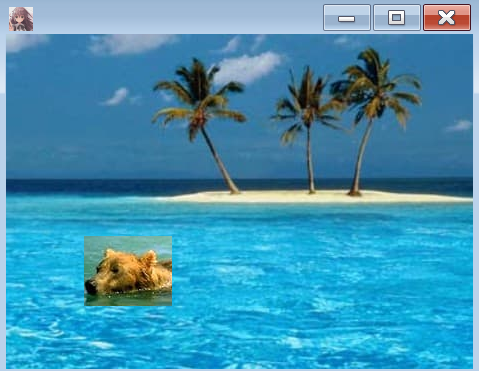
\includegraphics[width=6cm,height=4cm]{rect2}
		
		\caption{结果} \label{rect2.label}
	\end{center}
\end{figure}

  选择多边形区域时

\begin{figure}[H]
	\begin{center}
		
		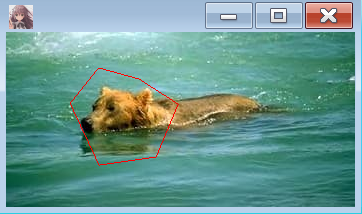
\includegraphics[width=6cm,height=4cm]{poly1}
		
		\caption{所选区域} \label{poly1.label}
	\end{center}
\end{figure}

\begin{figure}[H]
	\begin{center}
		
		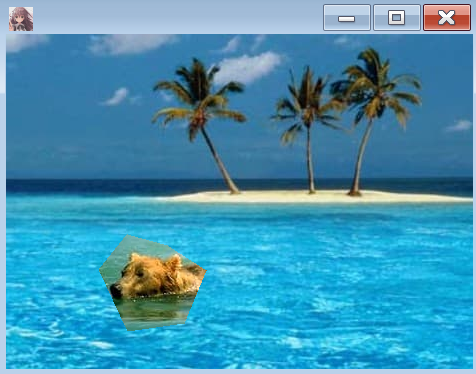
\includegraphics[width=6cm,height=4cm]{poly2}
		
		\caption{结果} \label{poly2.label}
	\end{center}
\end{figure}

  自由绘制区域时

\begin{figure}[H]
	\begin{center}
		
		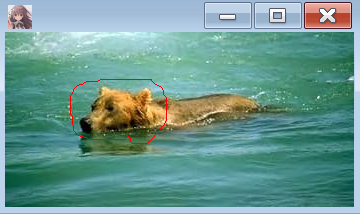
\includegraphics[width=6cm,height=4cm]{free1}
		
		\caption{所选区域} \label{free1.label}
	\end{center}
\end{figure}

\begin{figure}[H]
	\begin{center}
		
		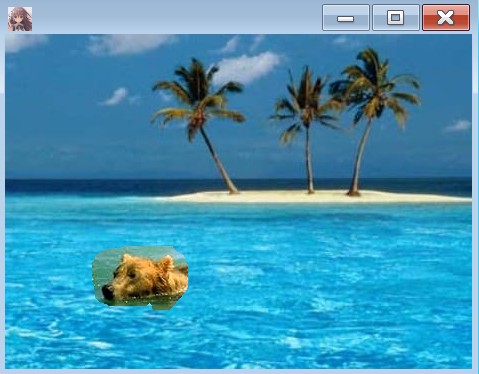
\includegraphics[width=6cm,height=4cm]{free2}
		
		\caption{结果} \label{free2.label}
	\end{center}
\end{figure}
    
        \subsubsection{内部梯度与混合梯度的对比}
        
        下面是使用两种梯度方法得到的结果。可以明显看出,混合梯度是更优一些的
        
      \begin{figure}[H]
      	\begin{center}
      		
      		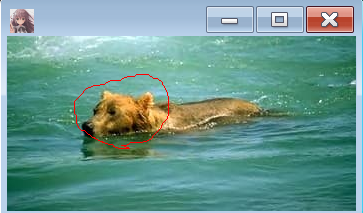
\includegraphics[width=6cm,height=4cm]{duibi1}
      		
      		\caption{所选区域} \label{duibi1.label}
      	\end{center}
      \end{figure}
        
        \begin{figure}[H]
        	\begin{center}
        		
        		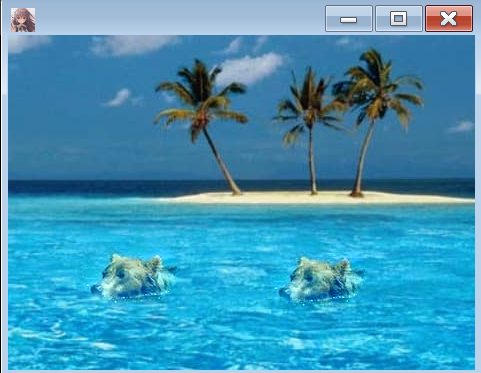
\includegraphics[width=6cm,height=4cm]{duibi2}
        		
        		\caption{结果:左边为内部梯度,右边为混合梯度} \label{duibi2.label}
        	\end{center}
        \end{figure}
        
            \subsubsection{最终结果}
            
          \begin{figure}[H]
        	\begin{center}
        		
        		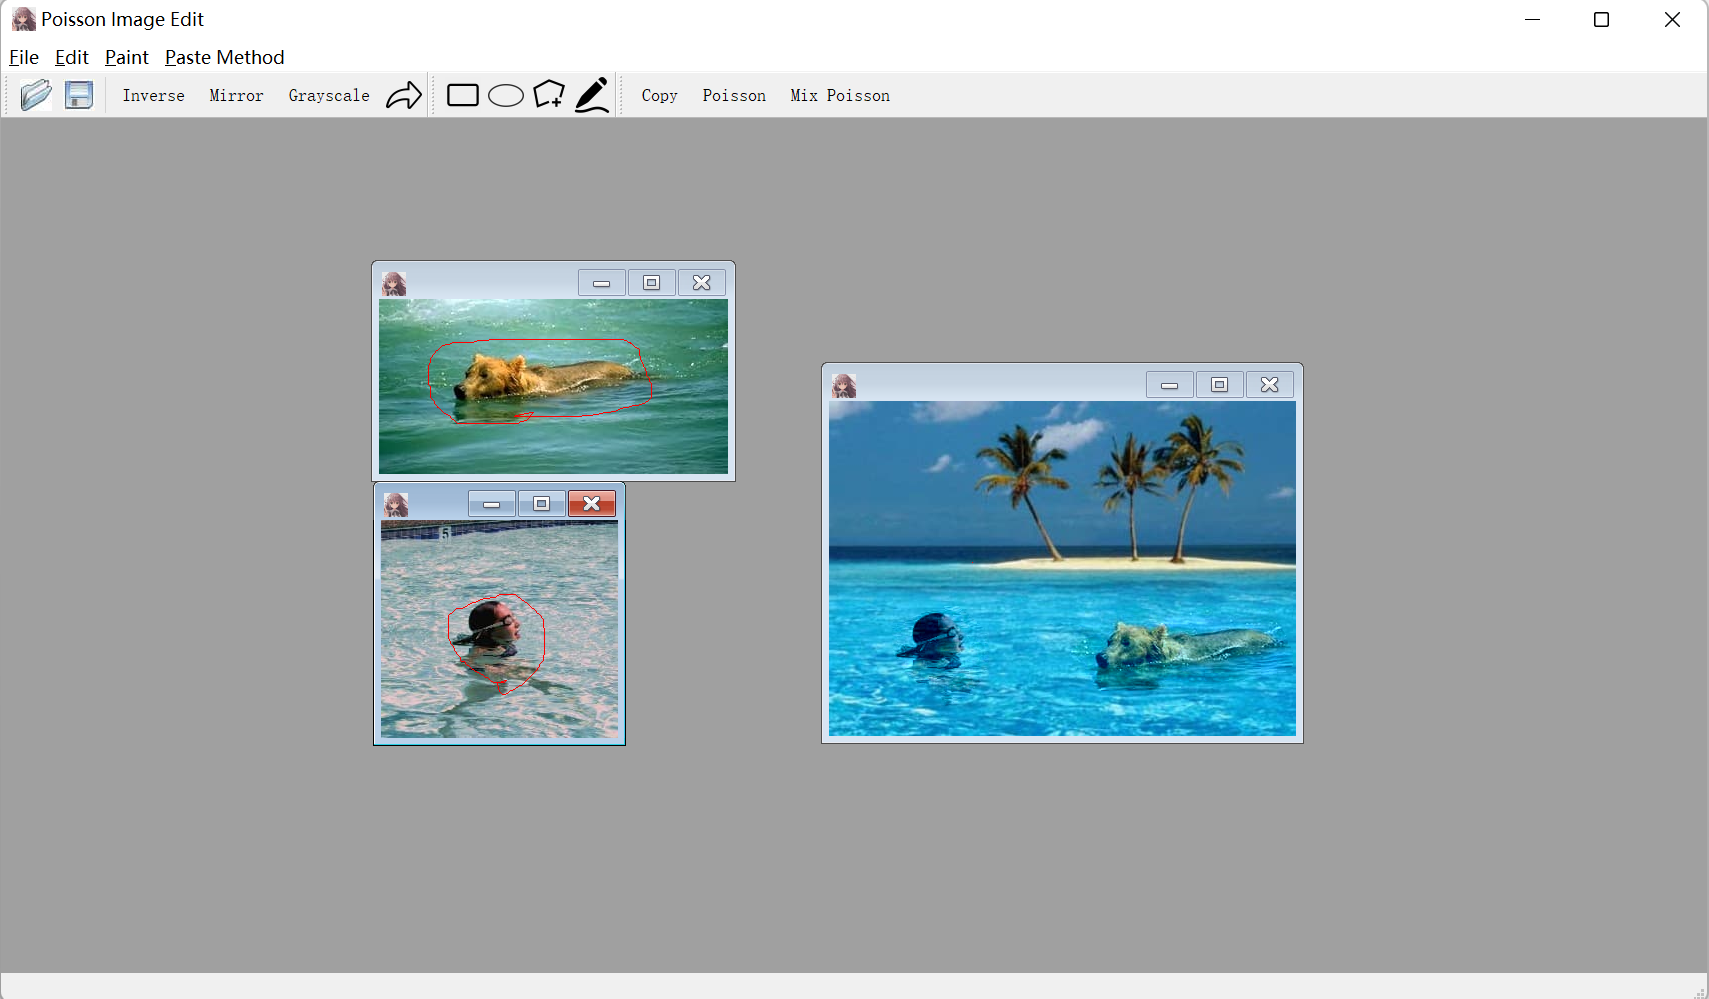
\includegraphics[width=13cm,height=8cm]{zuizhong}
        		
        		\caption{最终得到的结果} \label{zuizhong.label}
        	\end{center}
        \end{figure}
		

	
	
	\section{总结与讨论}
	
    
     \subsection{问题与不足}
     
     \begin{itemize}
     	\item 对于较大的图片,拖动时所需时间较长,效果不好
     \end{itemize}
 
    \begin{itemize}
 	\item 存在内存泄漏问题,不过貌似是因为opencv的mat库引起的
    \end{itemize}

    \begin{itemize}
	\item 程序的交互性和鲁棒性还可以做的更好些,时间问题来不及优化了
    \end{itemize}


  \subsection{反思}
  
   \begin{itemize}
  	\item 配置环境时一定要注意对应的版本!!因为本课程是2020年的,我自己一开始用的VS2022+opencv4.7.0在配置时踩了很多坑
  \end{itemize}

 \begin{itemize}
	\item 构建好项目可能会出现缺少opencv\_world470.dll的问题,可以利用网络资源来解决,如CSDN、ChatGPT等
\end{itemize}

 \begin{itemize}
	\item 特别注意OpenCV mat的行列问题!!
\end{itemize}

	
	
	
	
	
	





\begin{thebibliography}{99}
		\bibitem{PIE}
		Perez, Patrick. "Poisson Image Editing." ACM Transactions on Graphics (TOG), vol. 22, no. 3, 2003, pp. 313-318.
\end{thebibliography}
	
\end{document}